\section{Materials}
\subsection{Dataset}

Trong đồ án nghiên cứu lần này, nhóm sử dụng các bộ dữ liệu thời gian thực về giá của 3 loại tiền ảo phổ biến là Bitcoin (BTC), Binance (BNB) và Ethereum (ETH) từ ngày 01/03/2019 đến ngày 17/02/2024. Dữ liệu có 7 cột tượng trưng cho 7 thuộc tính mô tả một giao dịch, bao gồm Date, Open, High, Low, Close, Adj Close, Volume. Vì mục tiêu là dự báo giá kết phiên nên chỉ có dữ liệu liên quan đến cột “Close” mới được xử lý.

\subsection{Descriptive Statistics}
\begin{table}[H]
  \centering
  \caption{BTC, BNB, ETH’s Descriptive Statistics}
\begin{tabular}{|c|c|c|c|}
    \hline
     & BTC & BNB & ETH \\ \hline
     Count & 1815 & 1815 & 1815 \\ \hline
     Mean & 25794,936 & 204,769 & 1477,916\\ \hline
     Std & 15956,337 & 165,991 & 1156,45765\\ \hline
     Min & 3761,557 & 6,963 & 110,606\\ \hline
     25\% & 10251,123 & 23,650 & 255,537\\ \hline
     50\% & 23471,871 & 237,140 & 1567,846\\ \hline
     75\% & 38351,752 & 310,200 & 2120,294\\ \hline
     Max & 67566,828 & 634,550 & 4812,087\\ \hline
\end{tabular}
\end{table}

Theo bảng thống kê mô tả, trong ba loại tiền ảo, Bitcoin (BTC) có giá trị trung bình cao nhất với mức 25794.936 USD. BTC cũng cho thấy sự biến động giá lớn nhất so với Binance Coin (BNB) và Ethereum (ETH) do độ lệch chuẩn của nó (Std = 15956.337) lớn hơn nhiều so với các loại tiền ảo khác.Về các phân vị, BTC, ETH, và BNB đều có sự khác biệt rõ rệt, có thể thấy rằng ETH và BNB có mức trung bình và mức giá ở các phân vị thấp hơn so với BTC, nhưng ETH lại có xu hướng giá gần với BTC hơn so với BNB. Nhìn chung, BTC là loại tiền ảo có giá trị và độ biến động cao nhất, ETH có sự biến động vừa phải và giá trị trung bình, trong khi BNB có sự ổn định và giá trị thấp nhất trong ba loại tiền ảo này.

\begin{figure}[H]
    \centering
    \begin{minipage}{0.23\textwidth}
    \centering
    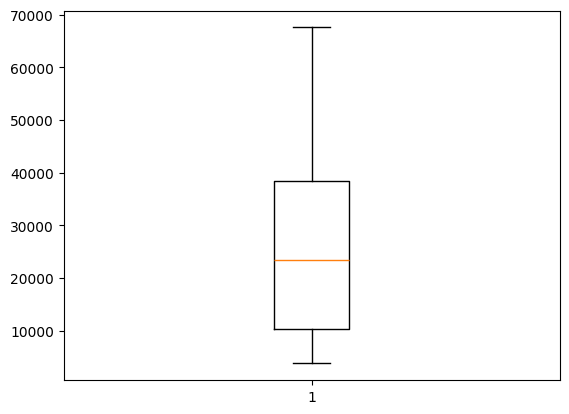
\includegraphics[width=1\textwidth]{bibliography/pictures/BTCboxplot.png}
    \caption{Biểu đồ boxplot về giá đóng phiên của Bitcoin}
    \label{fig:1}
    \end{minipage}
    \hfill
    \begin{minipage}{0.23\textwidth}
    \centering
    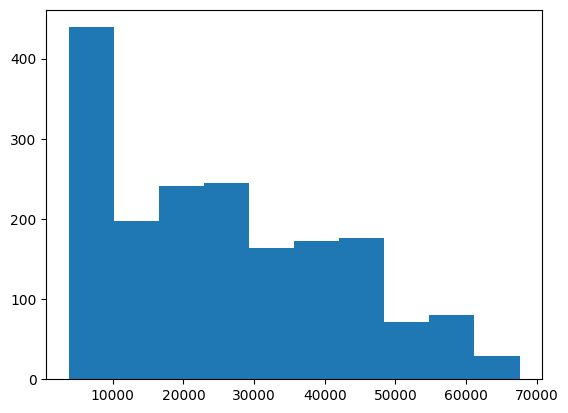
\includegraphics[width=1\textwidth]{bibliography/pictures/BTChistogram.png}
    \caption{Biểu đồ histogram về giá đóng phiên của Bitcoin}
    \label{fig:2}
    \end{minipage}
\end{figure}

\begin{figure}[H]
    \centering
    \begin{minipage}{0.23\textwidth}
    \centering
    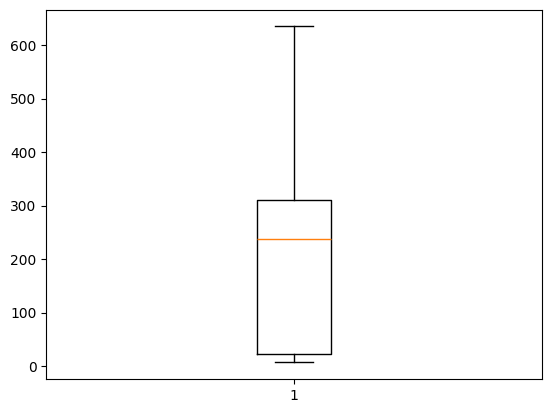
\includegraphics[width=1\textwidth]{bibliography/pictures/BNBboxplot.png}
    \caption{Biểu đồ boxplot về giá đóng phiên của Binance}
    \label{fig:1}
    \end{minipage}
    \hfill
    \begin{minipage}{0.23\textwidth}
    \centering
    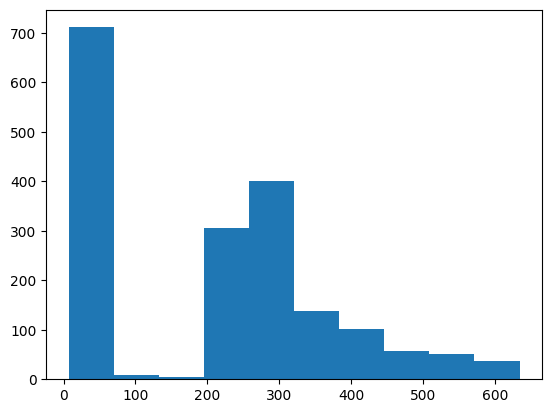
\includegraphics[width=1\textwidth]{bibliography/pictures/BNBhistogram.png}
    \caption{Biểu đồ histogram về giá đóng phiên của Binance}
    \label{fig:2}
    \end{minipage}
\end{figure}

\begin{figure}[H]
    \centering
    \begin{minipage}{0.23\textwidth}
    \centering
    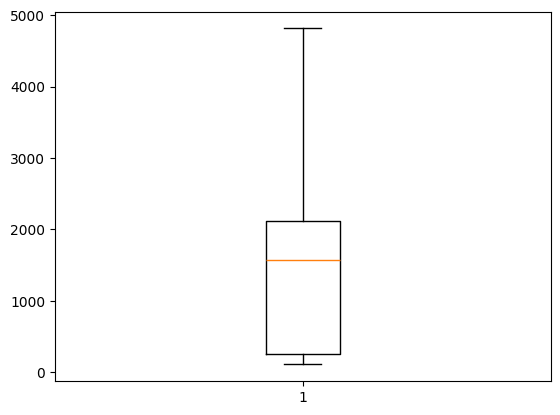
\includegraphics[width=1\textwidth]{bibliography/pictures/ETHboxplot.png}
    \caption{Biểu đồ boxplot về giá đóng phiên của Ethereum}
    \label{fig:1}
    \end{minipage}
    \hfill
    \begin{minipage}{0.23\textwidth}
    \centering
    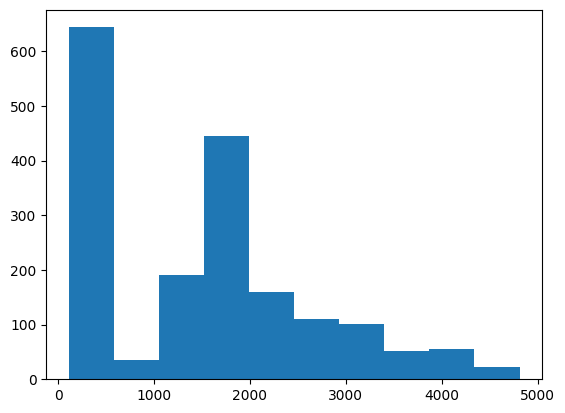
\includegraphics[width=1\textwidth]{bibliography/pictures/ETHhistogram.png}
    \caption{Biểu đồ histogram về giá đóng phiên của Ethereum}
    \label{fig:2}
    \end{minipage}
\end{figure}

Từ hình trên, ta thấy giá của ba loại tiền ảo BNB, BTC và ETH đều có xu hướng lệch phải. Biểu đồ hộp của BNB cho thấy giá trị khá đồng đều và ít biến động, với hộp có kích thước nhỏ và đường râu không kéo dài xa. Ngược lại, biểu đồ hộp của BTC thể hiện sự phân tán và biến động lớn nhất với hộp có kích thước lớn và đường râu kéo dài xa, đặc biệt là phía trên, cho thấy nhiều giá trị ngoại lệ cao. ETH cũng có sự phân tán lớn nhưng ít hơn BTC, với hộp có kích thước tương đối lớn và đường râu kéo dài. Biểu đồ tần suất của cả ba loại tiền ảo cho thấy phần lớn giá trị tập trung ở mức giá thấp hơn, nhưng BTC và ETH có nhiều giá trị ngoại lệ, đặc biệt là BTC. Điều này cho thấy BNB có xu hướng ổn định hơn, trong khi BTC và ETH biến động nhiều hơn, với BTC là loại tiền ảo có biến động lớn nhất.